En el capítulo \ref{chap:CR3BP} se estudió el problema restringido circular de los tres cuerpos. Dos partículas primarias orbitando en un plano a velocidad constante respecto a su centro de masa y una tercera influenciada por las otras dos con una dinámica muy rica. Rica es por elementos como la sensibilidad al parámetro de masa (\ref{eq:3body_mu}), la sensibilidad a condiciones inciales cercanas, las trayectorias discriminadas por su constante de Jacobi, o los cinco puntos lagrangianos (\ref{eq:3body_lag}). Esta sección busca explotar el transporte de jets como se describe en el capítulo \ref{sec:jt} así como los indicadores y herramientas desarrolladas en \ref{sec:jt_indicators}. 

En este capítulo se buscan explotar las propiedades dinámicas encontradas en \ref{chap:CR3BP} con ayuda de las herramientas planteadas en \ref{chap:jt_indicators}. Se utilizará al tranporte de jets en varias perspectivas donde, por ejemplo, se lo tratará como un integrador de flujo cuyas condiciones iniciales no se saben con presición, una herramienta para encontrar las ecuaciones de primera variación y más, método para encontrar las máximas y mínimas expansiones de la vecindad de una condición inicial dada en el espacio de configuraciones

Este capítulo se divide como sigue: 
%...

%Algo con las 0VC, 
%Parametrización de la masa (no está jalando; chance lo mochamos)
%heatmaps..
%direcciones de mayor y menor contracción alrededor de un punto
%simplecticidad??????
%ξmax en algo que no sea ξgrid? 

\section{Parametrización de $\mu$}
Como se analizó en el capítulo \ref{sec:lag}, $L_i = L_i(\mu)$, es decir, los puntos de equilibrio del PC3C dependen todos del parámetro de masa del sistema. Los puntos $L_4(\mu)$ y $L_5(\mu)$ son de particular interés ya que, a diferencia de los otros tres, serán estables si $\mu \leq \mu_c$, donde $\mu_c$ es el parámetro crítico de la masa dada por \ref{eq:3.36}. 

El análisis de eigenvalores alrededor de los puntos singulares nos da cómo es la estabilidad de dichos puntos, sin embargo, también es interesante ver las soluciones cerca de $\mu_c$ ya que nos permitirá ver directamente en el flujo el comportamiento de estabilidad de la masa que visita a $L_4$ o $L_5$.

Para esto, se seguirá la filosofía de la sección \ref{sec:parametrizacion}, donde se agregará a las ecuaciones de movimiento la ecuación 
\begin{equation*}
 \dot{\mu} = 0.
\end{equation*}
Con esto, se hará un transporte en $\mu$, es decir, ésta se parametrizará como 
\begin{equation*}
 \mu = \mu_0 + \delta\mu
\end{equation*}   
donde $\delta\mu \in \pkr$ y, por tanto, $\mu \in \pkr$ también. Se introduce la notación $\phi_\mu(t;t_0,\xo)$ para referirse a este tipo de transporte. Tomando $\mu_0 = \mu_c \approx 0.0385$, se está en el límite entre la estabilidad y la divergencia alrededor de los puntos $L_4$ y $L_5$.

%FIGURA!
\begin{figure}
 \centering
 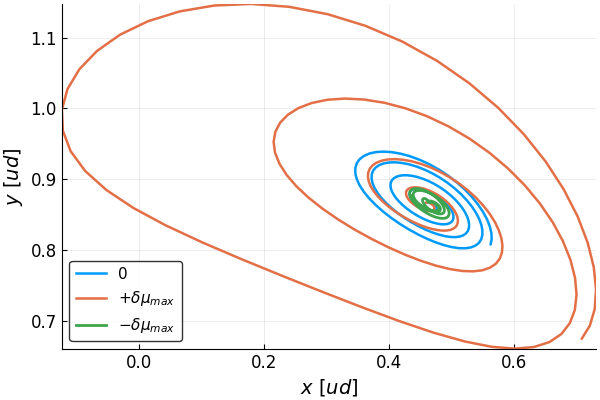
\includegraphics[width=0.8\linewidth]{flow_dmu}
 \caption{Espacio de configuraciones para $\phi_\mu$ con variaciones $\delta\mu = 0$ (azul), $\delta\mu = \delta\mu_{max}$ (naranja), y $\delta\mu = -\delta\mu_{max}$ (verde), donde $\delta\mu_{max} = \xi_{max}(\phi_\mu) \approx 0.00329$. Para el transporte se usó un jet de orden $n=18$ con condiciones iniciales $\left( L_{4_x}, L_{4_y} + \Delta y, 0, 0, \mu \right)$.}
 \label{fig:flow_dmu}
\end{figure}

Para hacer el transporte, tomaremos como condición inicial a $\xo = \left( L_{4_x}, L_{4_y} + \Delta y, 0, 0, \mu \right)$ con $\Delta y = 7\times 10^{-4}$ para no estar exáctamente en el punto fijo. Las variaciones de $\delta\mu$ estarán acotadas por el tamaño máximo de vecindad (\ref{eq:ximax}), es decir, $\delta\mu \leq \lvert \xi_{max}(\phi_\mu) \rvert$. Se puede ver en la figura \ref{fig:flow_dmu} una integración a $40$ unidades temporales, que equivalen a unos $X$ años. Se observa cómo para $\delta \mu > 0$, las soluciones se alejan cada vez más de $L_4$, mientras que para $\delta \mu < 0$ se queda en cierta localidad.

\section{Colisión de asteroides}

%%% Choro acerca de dos asteroides colisionando. %%% 

%%% Chorito acerca de cómo 4 masas es lo mismo que 3. (usando la masa de apohpis por ejemplo... %%%

%Hay en promedio $X$ objetos celestes orbitando a la Tierra 

%Hace 65 millones de años no existían métodos computacionales para determinar la trayectoria de las posibles colisiones de asteroides  con el planeta Tierra. ¿Qué sucedió?, los dinosaurios se extinguieron \cite{}. Hoy en día conocemos (o creemos conocer) las leyes que gobiernan la dinámica del sistema solar y los cuerpos que lo visitan así como métodos que resuelven dicha dinámica. Posiblemente no podamos detener el impacto, pero podemos intentar prepararnos para dicho suceso con varios años de anticipación. Por esto, es importante conocer el riesgo que tiene un objeto celeste de impactar con la Tierra, y el transporte de Jets es una muy buena herramienta para analizar dicha posibilidad. 

%con velocidad $\mathbf{v}_{a_1}(t_0) + \delta\mathbf{v}_{a_1}(t_0)$

Sean $a_1$ y $a_2$ dos asteroides con la misma energía de Jacobi alrededor de la masa primaria mayor. Inicialmente, éstos se encuentran a $\mathbf{x}_{a_1}(t_0) + \delta\mathbf{x}_{a_1}(t_0)$  y $\mathbf{x}_{a_2}(t_0) + \delta\mathbf{x}_{a_2}(t_0)$, respectivamente, donde $\delta\mathbf{x}_{a_i} \in \pkk{n}{2}$. La variación en cada condición representa el error de medición de éstos. Por tomar una referencia, tomemos la incertidumbre en el orden de los datos del asteroide Apophis en los años $2012 - 2028$ cite{Desmars2013}, donde definimos $\Delta_{max} := 350 $ km como la incertidumbre máxima para los asteroides.

%FIGURA!
\begin{figure}
 \centering
 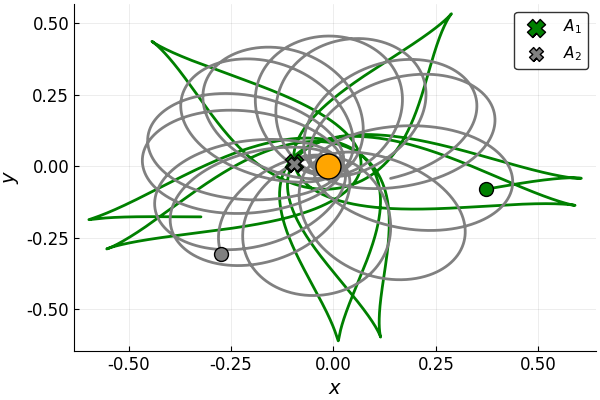
\includegraphics[width=0.7\linewidth]{asteroid_collision_nominal_integration}
 \caption{Integración nominal a $T=10 \approx $ unidades temporales, donde $\mathbf{q}_{a_1}(t_0) = \left( -0.373098, -0.0804321, 1.21995, \dot{y}_{a_1} \left( x_{a_1}(t_0), y_{a_1}(t_0), \dot{x}_{a_1}(t_0), C_J \right) \right)$ 
 y $\mathbf{q}_{a_2}(t_0) = \left( -0.27324, -0.307896, -0.307576, \dot{y}_{a_2} \left( x_{a_2}(t_0), y_{a_2}(t_0), \dot{x}_{a_2}(t_0), C_J \right) \right)$. El círculo naranja representa a $M_1$, y los círculos verde y gris a $\mathbf{q}_{a_1}(t_0)$ y $\mathbf{q}_{a_2}(t_0)$, respectivamente. La zona de mayor acercamiento se marca con cruces, donde en ésta, la distancia entre los asteroides es de $0.00348 \approx 1341$ km.}
 \label{fig:asteroid_collision_nominal_integration}
\end{figure}

La figura \ref{fig:asteroid_collision_nominal_integration} muestra la trayectoria nominal de $a_1$ y $a_2$ para condiciones iniciales con energía $C_J = -1.81252 < C_J(L_1)$. En esta integración, la mínima distancia entre ambos cuerpos es de $0.00348$ que representa unos $1341$ kilómetros. Sin embargo, aunque para esta condición particular los asteroides no chocan, es posible que sí lo hagan dentro de una incertidumbre de radio $\Delta_{max}$. Esto se puede hacer con el transporte de jets de la siguiente manera: 

\begin{itemize}
 \item Hacer una integración nominal de dos asteroides con energías similares o que se sepa que pueden tener riesgo de colisión.
 
 \item Encontrar las coordenadas $\mathbf{q}_{a_i}^{(col)}$ donde la distancia entre $a_1$ y $a_2$ es mínima.
 
 \item Hacer TJ alrededor de las condiciones encontrada en el punto anterior.
 
 \item Evaluar una distribución de $N$ puntos en la bola $\delta\mathbf{x}_i \leq \Delta_{max}$ alrededor de $\mathbf{q}_{a_i}^{(col)}$ para ambos asteroides y guardarla.
 
 \item Definir una distancia $D_{col}$ para la cual los asteroides chocarían y determinar qué puntos de la distribución quedan debajo de ésta.
 
 \item Determinar la probabilidad de impacto $\mathcal{P}$ como la cantidad de veces puntos que quedan debajo de $D_{col}$ respecto al número de trayectorias totales $N^2$; así
 \begin{equation} 
 \mathcal{P} = \frac{\norm{\mathbf{x}_{a_1} - \mathbf{x}_{a_2} }    \leq D_{col} }{N^2}.
 \end{equation}
\end{itemize}

%FIGURA!
\begin{figure}
 \centering
 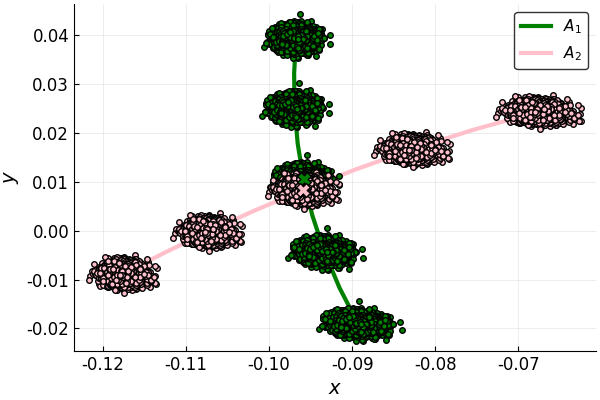
\includegraphics[width=0.7\linewidth]{asteroid_collision_distribution}
 \caption{Transporte de jets de orden $4$ alrededor de $\mathbf{q}_{a_i}^{(col)}$ (cruces en la figura) donde los cúmulos son la distribución de radio $\delta\mathbf{x}_{a_i} \leq 350$ km evaluadas en el polinomio resultante del transporte. Para el método sólo se toman los cúmulos donde se encuentra $\mathbf{q}_{a_i}^{(col)}$, pero la figura busca ilustrar una sección de la trayectoria de los asteroides.}
 \label{fig:asteroid_collision_distribution}
\end{figure}

La figura \ref{fig:asteroid_collision_distribution} muestra una distribución normal de $7000$ puntos\footnote{$7000$ ya convergen a una probabilidad cuyas cifras significativas no afectan el redondeo de la tabla \ref{table:collision_table}.} evaluados en el transporte alrededor de $\mathbf{q}_{a_i}^{(col)}$ para $i = \{1,2\}$. La probabilidad de impacto dependerá del tamaño que tengan los asteroides, la cual se presenta en la tabla \ref{table:collision_table}. Se presenta en la figura \ref{fig:asteroid_collision_histogram} la distribución de distancias entre ambos asteroides en la zona de riesgo de colisión. Aún cuando $D_{col}$ e incluso $\Delta_{max}$ quedan debajo del escenario más posible en la distribución, la probabilidad de impacto es suficientemente grande para no ser ignorada en los asteroides de mayor dimensión.

%TABLA!
\begin{table}[h!]
\centering
\begin{tabular}{c|c|c}
\toprule
\textbf{$ D_{col}$ [ km ]} & \textbf{$\mathcal{P}$ [ $\%$ ]} & \textbf{Colisiones [ $ \# $ ]} \\ \cmidrule(l){1-3} 
\textbf{$0.5$} &   $3.7 \times 10^{-5}$   & $18$          \\
\textbf{$5$}   &   $0.0048$               & $2356$        \\
\textbf{$30$}  &   $0.172$                & $84,609$     \\
\textbf{$150$} &   $4.357$                & $2,135,173$   \\ \bottomrule 
\end{tabular}
\caption{Número de colisiones y riesgo de choque para asteroides de distintas dimensiones.}
\label{table:collision_table}
\end{table}

%FIGURA!
\begin{figure}
 \centering
 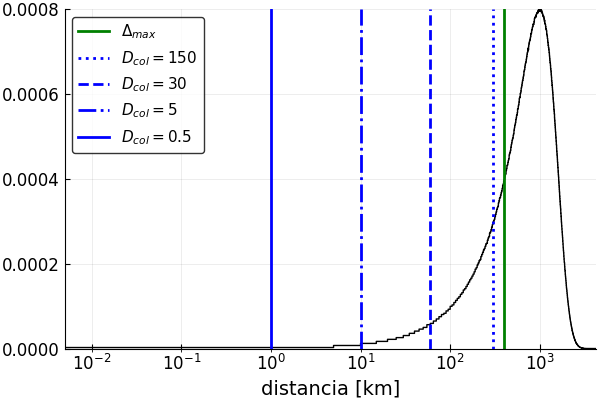
\includegraphics[width=0.7\linewidth]{asteroid_collision_histogram}
 \caption{Distribución normalizada de distancias entre $a_1$ y $a_2$ cerca del punto de posible dadas $7000$ variaciones iniciales alrededor de $\mathbf{q}_{a_1}^{col}$ y $\mathbf{q}_{a_2}^{col}$. Las líneas verticales muestran los valores usados en la tabla \ref{table:collision_table}.}
 \label{fig:asteroid_collision_histogram}
\end{figure}


Algo relevante al hacer transporte de jets es la presición de éste. Se encuentra que $\xi_{max}(\phi_{a_1}) = 0.0022 \approx 865 \ km \gg \Delta_{max}$\footnote{$\xi_{max}(\phi_{a_2})$ es prácticamente igual a $\xi_{max}(\phi_{a_1})$.}, por lo que se tiene bastante confianza en la precisión de las evaluaciones de la distribución. De hecho, al tomar una serie de variaciones $\norm{\delta\mathbf{x}_{a_i}} = \Delta_{max}$ y hacer la integración nominal de éstas, se encuentra que el error promedio respecto a éstas es del orden de $10^{-11} \approx 4 mm$, o sea, nada. Ésto se muestra en la figura \ref{fig:asteroid_jt_vs_nominal}.

%FIGURA!
\begin{figure}
 \centering
 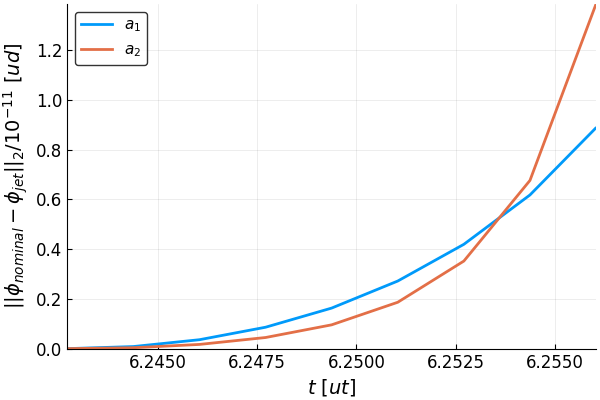
\includegraphics[width=0.7\linewidth]{asteroid_jt_vs_nominal}
 \caption{Promedio de la distancia entre la integración nominal y el transporte de jets para $500$ condiciones iniciales con variación $\norm{\delta\mathbf{x}_{a_1}} = \norm{\delta\mathbf{x}_{a_1}} = \Delta_{max}$.}
 \label{fig:asteroid_jt_vs_nominal}
\end{figure}

Así, ilustramos el método de posible colisión entre asteroides, donde se estableció la probabilidad de impacto para diferentes zonas de colisión. El transporte de jets permitió encontrar dichas probabilidades ya que en éste, simplemente hubo que evaluar la distribución de variaciones iniciales en un radio dado. Éste método es generalizable a cualquier sistema donde exista alguna incertidumbre en las condiciones iniciales. Sin embargo, hay que tener claro que el transporte de jets no es muy preciso para integraciones muy largas ni para vecindades muy grandes. En este ejemplo, el radio de las variaciones eran $0.46$ veces más pequeñas que $\xi_{max}$. Además, se hizo la integración de jets cerca del punto de posible colisión para tener tiempo de integración cortos. 

%Mencionar adimensionalización del tiempo para ver cuánto implica 1 unidad temporal.